

\section{Houdini basics}


word\footnote{Explanation of the word.} that
ddjword\footnote{Explanation of the word.} that
jord\footnote{Explanation of the word.} that

You can find the source code on GitHub: \url{https://github.com/your-username/your-repository}.


\begin{figure}[H] 
    \centering
    \begin{subfigure}[b]{0.49\textwidth}
        \centering
        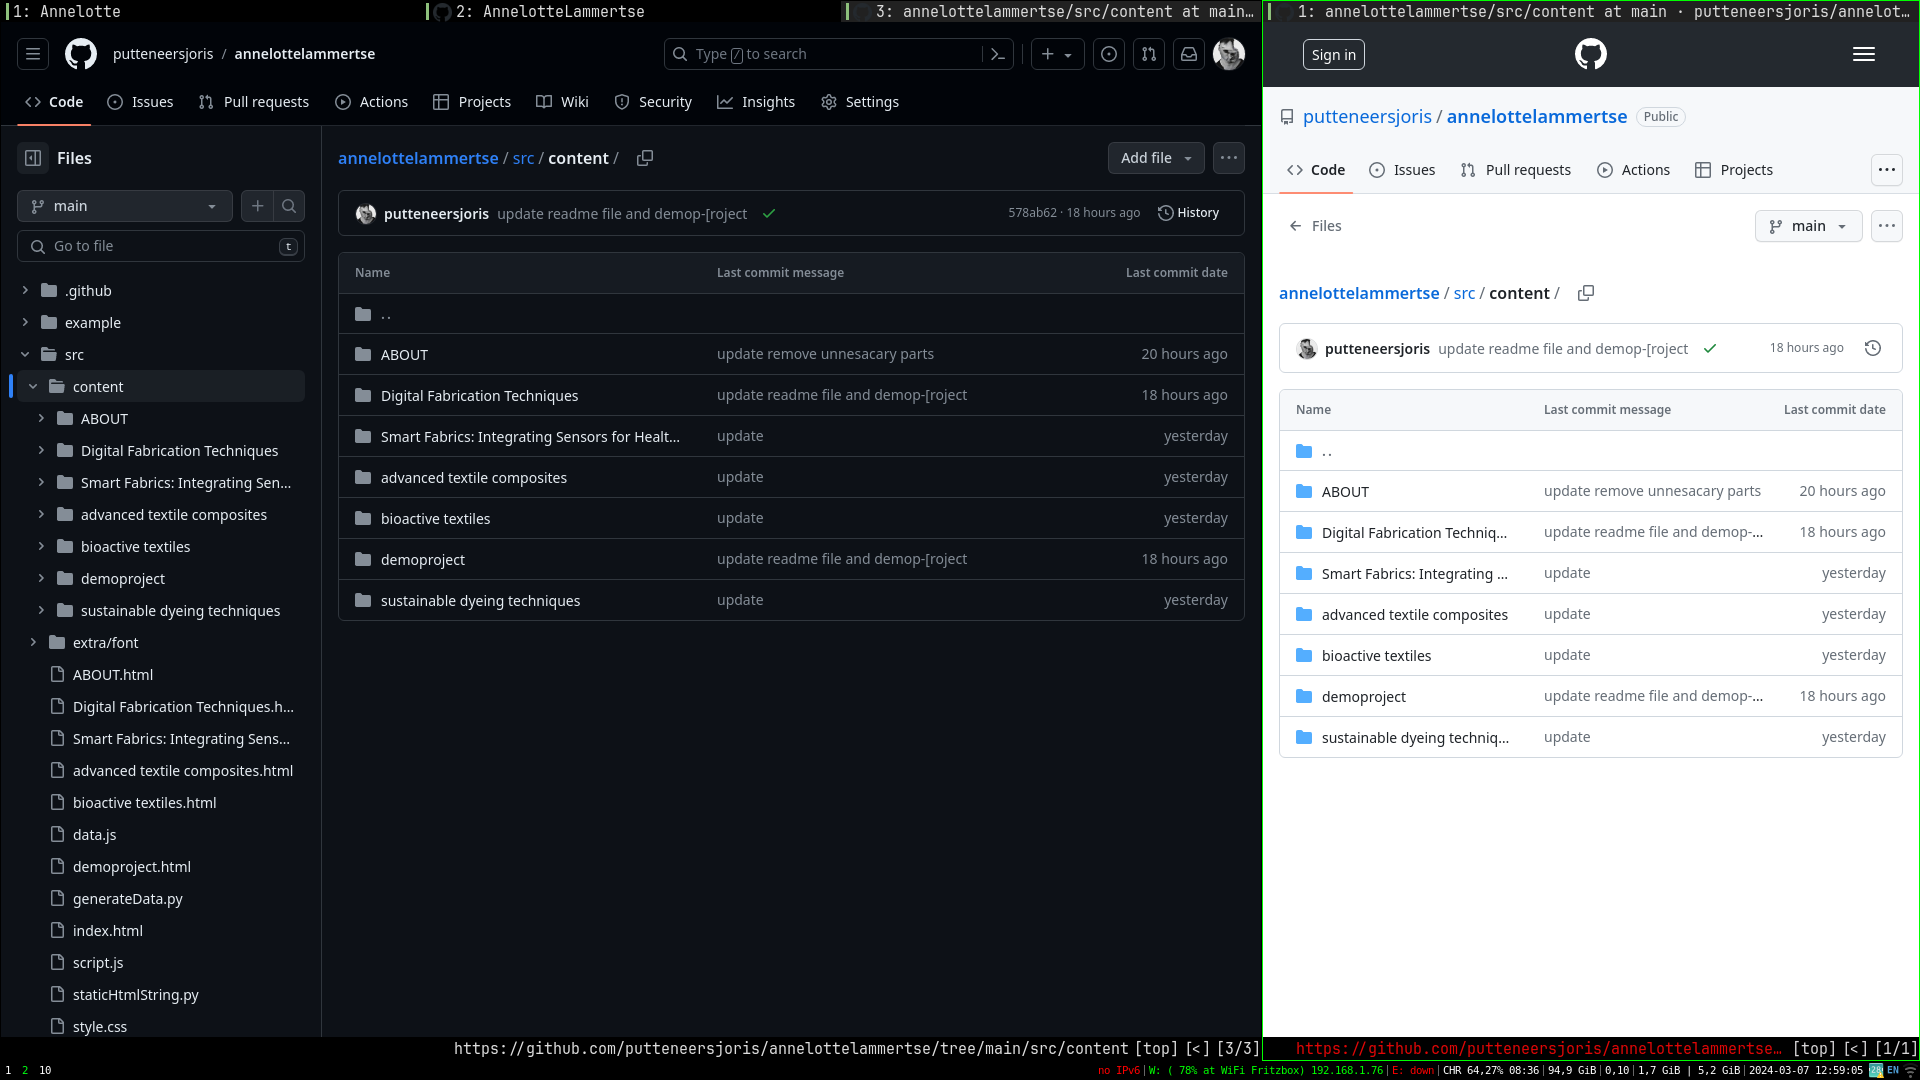
\includegraphics[width=1\textwidth]{sections/assignment_1/1.png}
        \caption{digital signal}
    \end{subfigure}
    \hfill
    \begin{subfigure}[b]{0.49\textwidth}
        \centering
        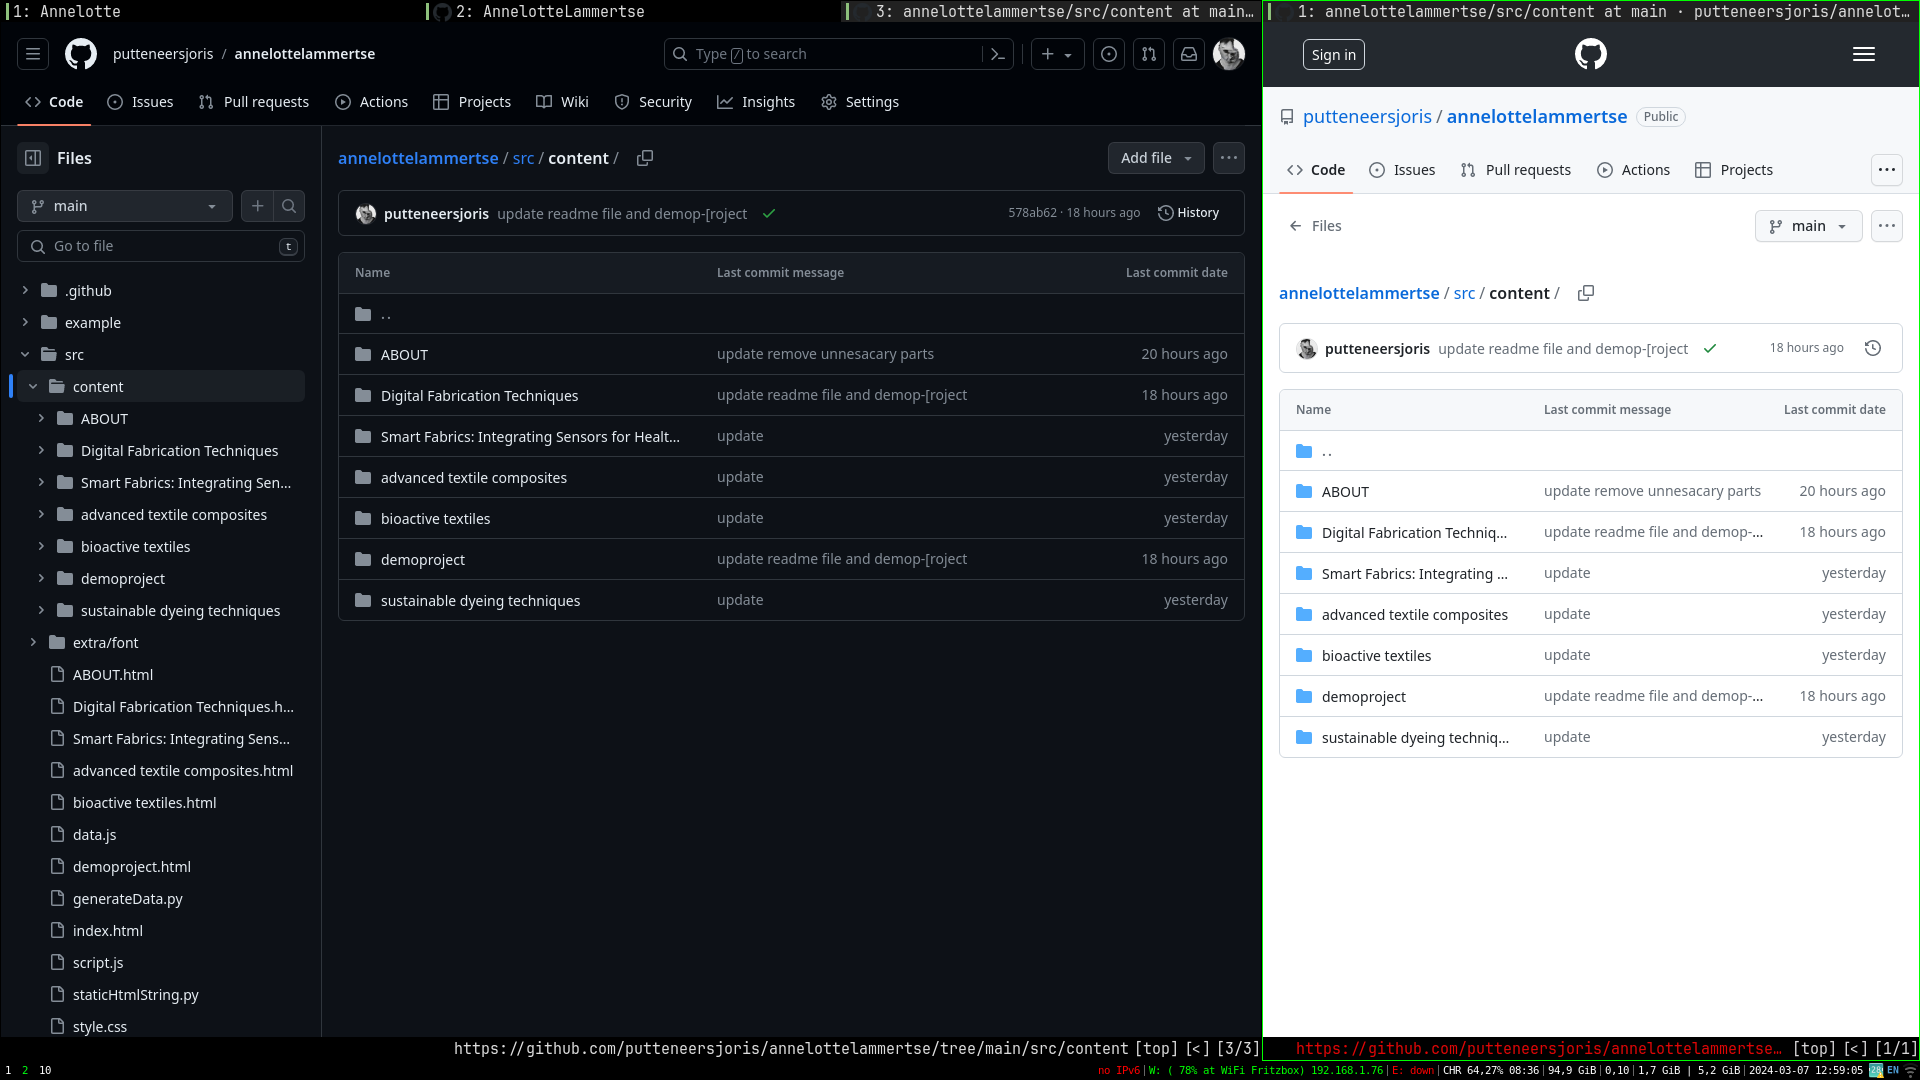
\includegraphics[width=1\textwidth]{sections/assignment_1/1.png}
        \caption{analog signali of the same signal that dispalyssi the same signal that dispalyssi the same signal that dispalyssi the same signal that dispalyssi the same signal that dispalyssi the same signal that dispalys} 
    \end{subfigure}
\end{figure}


\keywords{node / context / parameter / attribute / primitive /mitive mitive mitive mitive mitive  vertex / point / object / procedural / datatype}



